\documentclass[12pt]{article}
\usepackage{graphicx}
\usepackage{subcaption}
\usepackage{mwe}
\usepackage{amsmath}
\usepackage{mathtools}
\usepackage[]{mcode}
\usepackage{listings}
\usepackage{color} %red, green, blue, yellow, cyan, magenta, black, white

%\usepackage{lingmacros}
%\usepackage{tree-dvips}
%\usepackage{blindtext}
%\usepackage[utf8]{inputenc}

\newcommand{\norm}[1]{\left\lVert#1\right\rVert}
\newcommand{\abs}[1]{\left|#1\right|}
\renewcommand{\thesubsection}{\thesection.\alph{subsection}}

\begin{document}

\title{Assignment 2}
\author{Gudjon Einar Magnusson}

\maketitle


\section{} %% Problem 1

\subsection{} %% 1a

Figure \ref{fig_ut_pt} shows the function $u(t) = 1/(1.1 - cos t)$ and the polynomial interpolation $p(t)$ using 11 equidistant points.

The interpolation is performed using the functions \textit{cos\_transform} and \textit{inv\_cos\_transform}, shown below.

\noindent
\begin{minipage}{\linewidth}
\lstinputlisting{../cos_transform.m}
\end{minipage}

\noindent
\begin{minipage}{\linewidth}
\lstinputlisting{../inv_cos_transform.m}
\end{minipage}

\begin{figure}
    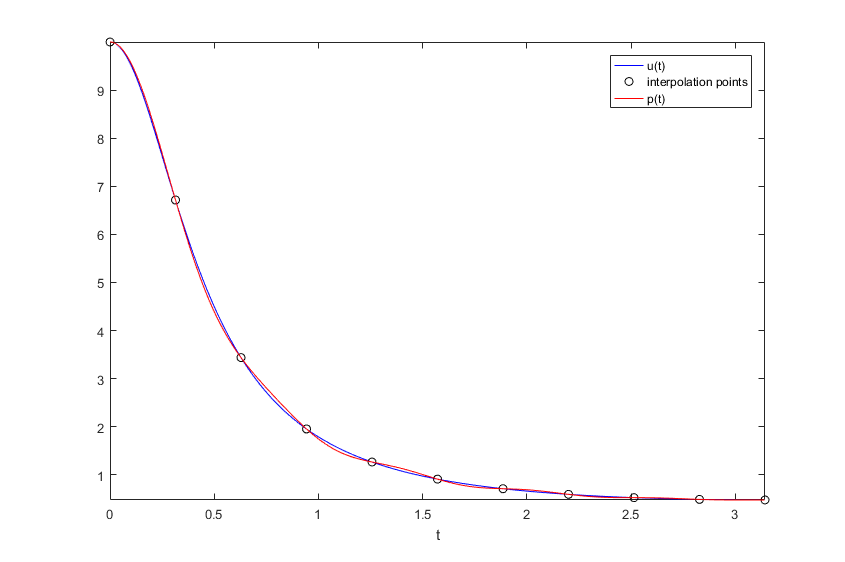
\includegraphics[width=0.6\linewidth]{ut_pt}
    \centering
    \caption{$u(t)$ and the interpolating polynomial $p(t) \in \mathcal{P}_{10}$. Using 11 equidistant nodes.}
    \label{fig_ut_pt}    
\end{figure}


\subsection{} %% 1b

Figure \ref{fig_pt_log_err} shows how the error $\norm{u-p_n}_{\infty}$ decays as $n$ increases. The Log of the error drops linearly which indicates exponential convergence.

Below you can see the output produced when estimating the error for $n = 2, 4, \ldots, 50$.
N is the order of the polynomial. E is the error estimate $E_n$. S is the slope between 
the points $(n-2, log E_{n-2}), (n, log E_n)$.

\begin{minipage}{\linewidth}
\begin{lstlisting}
N: 4   E: 1.6581      S: -0.45972
N: 6   E: 0.60969     S: -0.50024
N: 8   E: 0.2606      S: -0.42498
N: 10  E: 0.11235     S: -0.4207
N: 12  E: 0.046269    S: -0.44356
N: 14  E: 0.018576    S: -0.45631
N: 16  E: 0.0078078   S: -0.43337
N: 18  E: 0.0032452   S: -0.43898
N: 20  E: 0.001331    S: -0.44563
N: 22  E: 0.00054384  S: -0.4475
N: 24  E: 0.00022618  S: -0.43867
N: 26  E: 9.3312e-05  S: -0.44268
N: 28  E: 3.8287e-05  S: -0.44542
N: 30  E: 1.5764e-05  S: -0.4437
N: 32  E: 6.5138e-06  S: -0.44189
N: 34  E: 2.6821e-06  S: -0.44366
N: 36  E: 1.1014e-06  S: -0.44502
N: 38  E: 4.5448e-07  S: -0.44258
N: 40  E: 1.8723e-07  S: -0.4434
N: 42  E: 7.7184e-08  S: -0.44308
N: 44  E: 3.1691e-08  S: -0.44508
N: 46  E: 1.3085e-08  S: -0.44228
N: 48  E: 5.3855e-09  S: -0.44387
N: 50  E: 2.2195e-09  S: -0.44322
\end{lstlisting}
\end{minipage}

\begin{figure}
    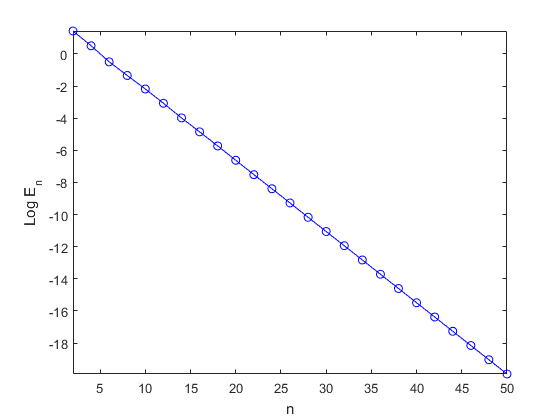
\includegraphics[width=.6\linewidth]{pt_log_err}
    \centering
    \caption{The error $\norm{u-p_n}_{\infty}$ drops exponentially as $n$ increases.}
    \label{fig_pt_log_err}
\end{figure}


\subsection{} %% 1c
Derp

\subsection{} %% 1d

Figure \ref{fig_vt_pt} shows the function $v(x) = \abs{x}^{1/3}$ and the polynomial interpolation $p(t)$ using 9 Chebyshev nodes.

\begin{figure}
    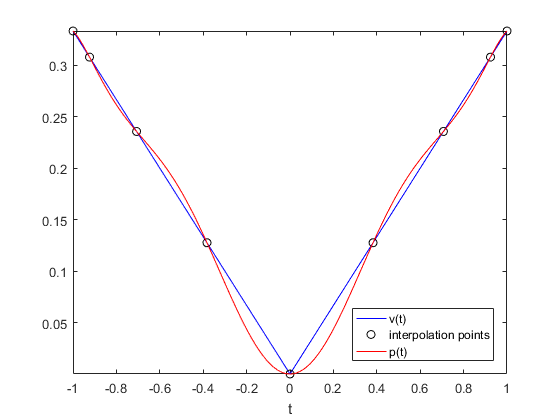
\includegraphics[width=.6\linewidth]{vt_pt}
    \centering
    \caption{$v(x)$ and the interpolating polynomial $p(x) \in \mathcal{P}_{8}$. Using 9 Chebyshev nodes.}
    \label{fig_vt_pt}
\end{figure}


\section{} %% Problem 2

\subsection{} %% 2a
The function \textit{interperr\_eq} approximates the function $u(x) = (1+30x^2)^{-1}$ with the interpolating polynomial $p_n(x)$ using $n+1$ equidistant nodes. Using Lagrange formula with equidistant nodes suffers from Runge's phenomenon. It oscillates far from the true value at the edges of the range.

Figure \ref{fig_eq_err_alpha} shows the error $\norm{u-p_n}_{\infty}$ goes down at first but then increases exponentially as $n$ increases. The oscillation get worse and worse as $n$ increases.

To roughly estimate the decay rate $\alpha$, I divided the range of $E$ with the range of $n$ to get a slope. Figure \ref{fig_eq_err_alpha} shows he line $log Ce^{\alpha n}$ using the estimate for $\alpha$ and it does satisfy the the condition $E_n \le Ce^{\alpha n}$.
In this case $\alpha = 0.29310$ and $C = 0.4$.

\noindent
\begin{minipage}{\linewidth}
\lstinputlisting{../interperr_eq.m}
\end{minipage}

\begin{figure}
    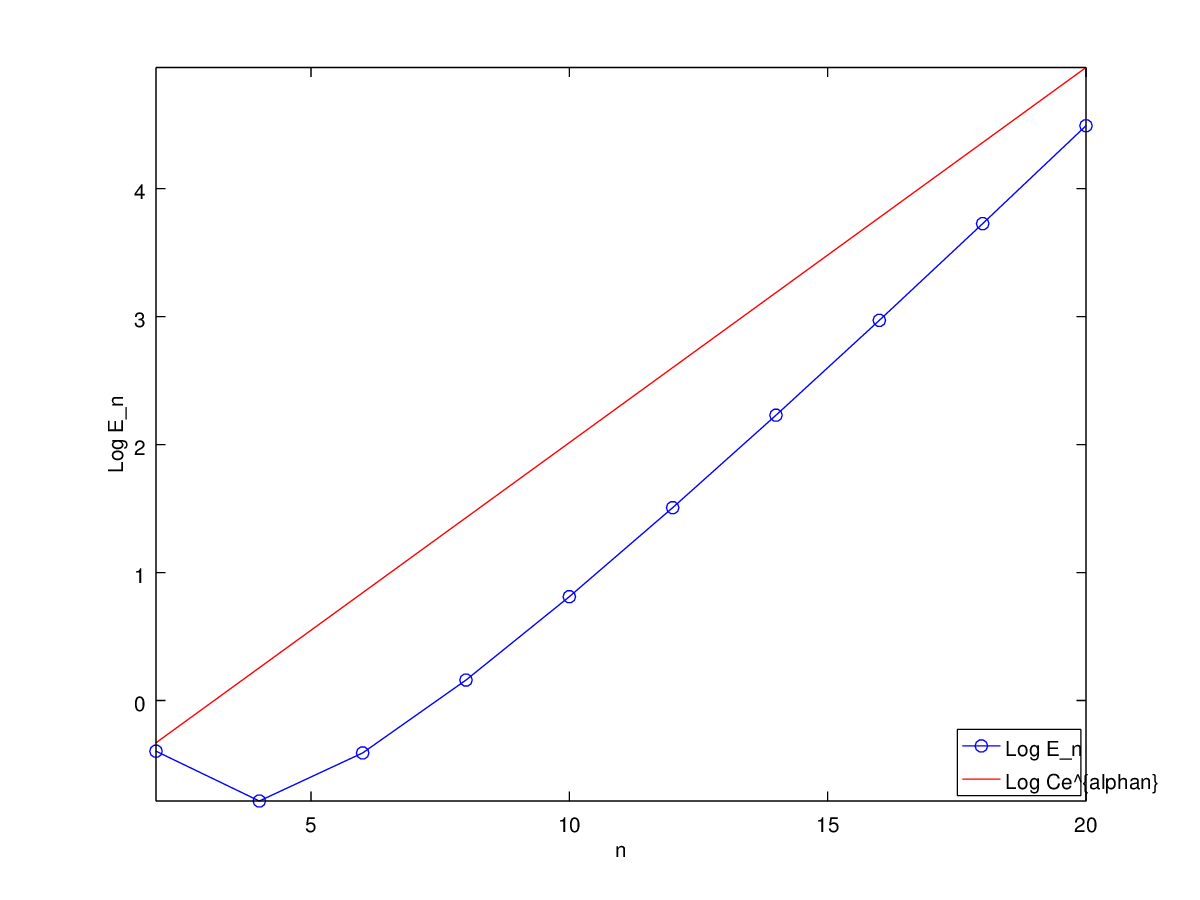
\includegraphics[width=.6\linewidth]{eq_err_alpha}
    \centering
    \caption{$Log E_n$ and a rough estimate of the decay rate $\alpha$}
    \label{fig_eq_err_alpha}
\end{figure}

\subsection{} %% 2b

The function \textit{interperr\_ch} approximates the function $u(x) = (1+30x^2)^{-1}$ with the interpolating polynomial $p_n(x)$ using $n+1$ Chebyshev nodes. By using Chebyshev nodes the oscillation issue is fixed. Nodes a placed closer together at the edges of the range.

Figure \ref{fig_ch_err_alpha} shows the error $\norm{u-p_n}_{\infty}$ decreases exponentially as $n$ increases.
It also shows a rough estimate for $\alpha$ as the line $log Ce^{\alpha n}$, it does satisfy the the condition $E_n \le Ce^{\alpha n}$.
In this case $\alpha = -0.18374$ and $C = 1.04$.

\noindent
\begin{minipage}{\linewidth}
\lstinputlisting{../interperr_ch.m}
\end{minipage}

\begin{figure}
    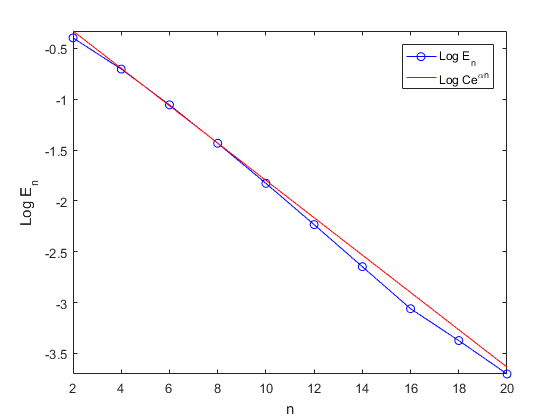
\includegraphics[width=.6\linewidth]{ch_err_alpha}
    \centering
    \caption{$Log E_n$ and a rough estimate of the decay rate $\alpha$}
    \label{fig_ch_err_alpha}
\end{figure}

\subsection{} %% 2c

% U1
\begin{minipage}{\linewidth}
\begin{lstlisting}
N: 4   E: 0.48476  S: -0.26463
N: 6   E: 0.42788  S: -0.30784
N: 8   E: 0.3902   S: -0.32043
N: 10  E: 0.36288  S: -0.32529
N: 12  E: 0.34177  S: -0.32863
N: 14  E: 0.32486  S: -0.32917
N: 16  E: 0.31085  S: -0.33019
N: 18  E: 0.29897  S: -0.33097
N: 20  E: 0.28859  S: -0.33527
\end{lstlisting}
\end{minipage}

% U2
\begin{minipage}{\linewidth}
\begin{lstlisting}
N: 4   E: 0.21655   S: -0.6285
N: 6   E: 0.1661    S: -0.65417
N: 8   E: 0.13736   S: -0.66042
N: 10  E: 0.11847   S: -0.66293
N: 12  E: 0.10496   S: -0.66444
N: 14  E: 0.094735  S: -0.66463
N: 16  E: 0.086682  S: -0.66528
N: 18  E: 0.080119  S: -0.66843
N: 20  E: 0.074692  S: -0.66581
\end{lstlisting}
\end{minipage}

\section{} %% Problem 3

\subsection{} %% 3a
\subsection{} %% 3b

\end{document}